

%..--..--..--..--..--..--..--..--..--..--..--..--..--..--..--..--..--..--..--..--..--..--..--..--..--..--..--..--..--..--..--..
%\subsubsection{$\pi$-{\sc Pews}  meta-model}\label{sec:pewsmetamodel}
%..--..--..--..--..--..--..--..--..--..--..--..--..--..--..--..--..--..--..--..--..--..--..--..--..--..--..--..--..--..--..--..

\pisodm  proposes intra-level transformation rules between $\pi$-use case to $\pi$-service process models, $\pi$-service process to $\pi$-service composition  models, as well as inter-level transformation rules between $\pi$-service composition to $\pi$-PEWS models. 
These rules are used to build a semi-automatic tool.
The transformations from CIM to PIM level models is not automatized, due to the informal nature of CIM level representations.
 
% _ . _ . _ . _ . _ . _ . _ . _ . _ . _ . _ . _ . _ . _ . _ . _ . _ . _ .
\subsection{From $\pi$-UseCase to the $\pi$-ServiceProcess}
% _ . _ . _ . _ . _ . _ . _ . _ . _ . _ . _ . _ . _ . _ . _ . _ . _ . _ .

The refinement of a (composite) $\pi$-Use Case model into a $\pi$-Service Process model is driven by the principle of expressing a set of $\pi$-use cases (i.e., use cases with constraints)   in terms of  a business process.
The resulting model consists of actions related by a control flow and contracts specifying NFPs. 

As defined by the $\pi$-ServiceProcess  meta-model (Figure~\ref{fig:CIM:serviceprocessmetamodel}) an {\sc Activity Service} consists of a composition of  entities of type {\sc Action}. 
Thus, every {\sf $\pi$-use case} is transformed into an {\sf Action} of the target $\pi$-Service Process model.  
Every {\sf Extend} relationship identified in a $\pi$-Use Case model is transformed into a  {\sf Fork node}\footnote{Notice that Fork nodes are used both to represent alternative and parallel execution. {\color{red} \sc Placido, please check this!}}.
If the {\sf Extend} relationship concerns just one {\sf use case}, it is transformed into an {\sf Action} inside one flow of the fork node. 
Otherwise, several  {\sf use cases} are transformed into different {\sf Actions} that belong to different flows departing from the fork node.   

%\begin{figure}
%\centering{
%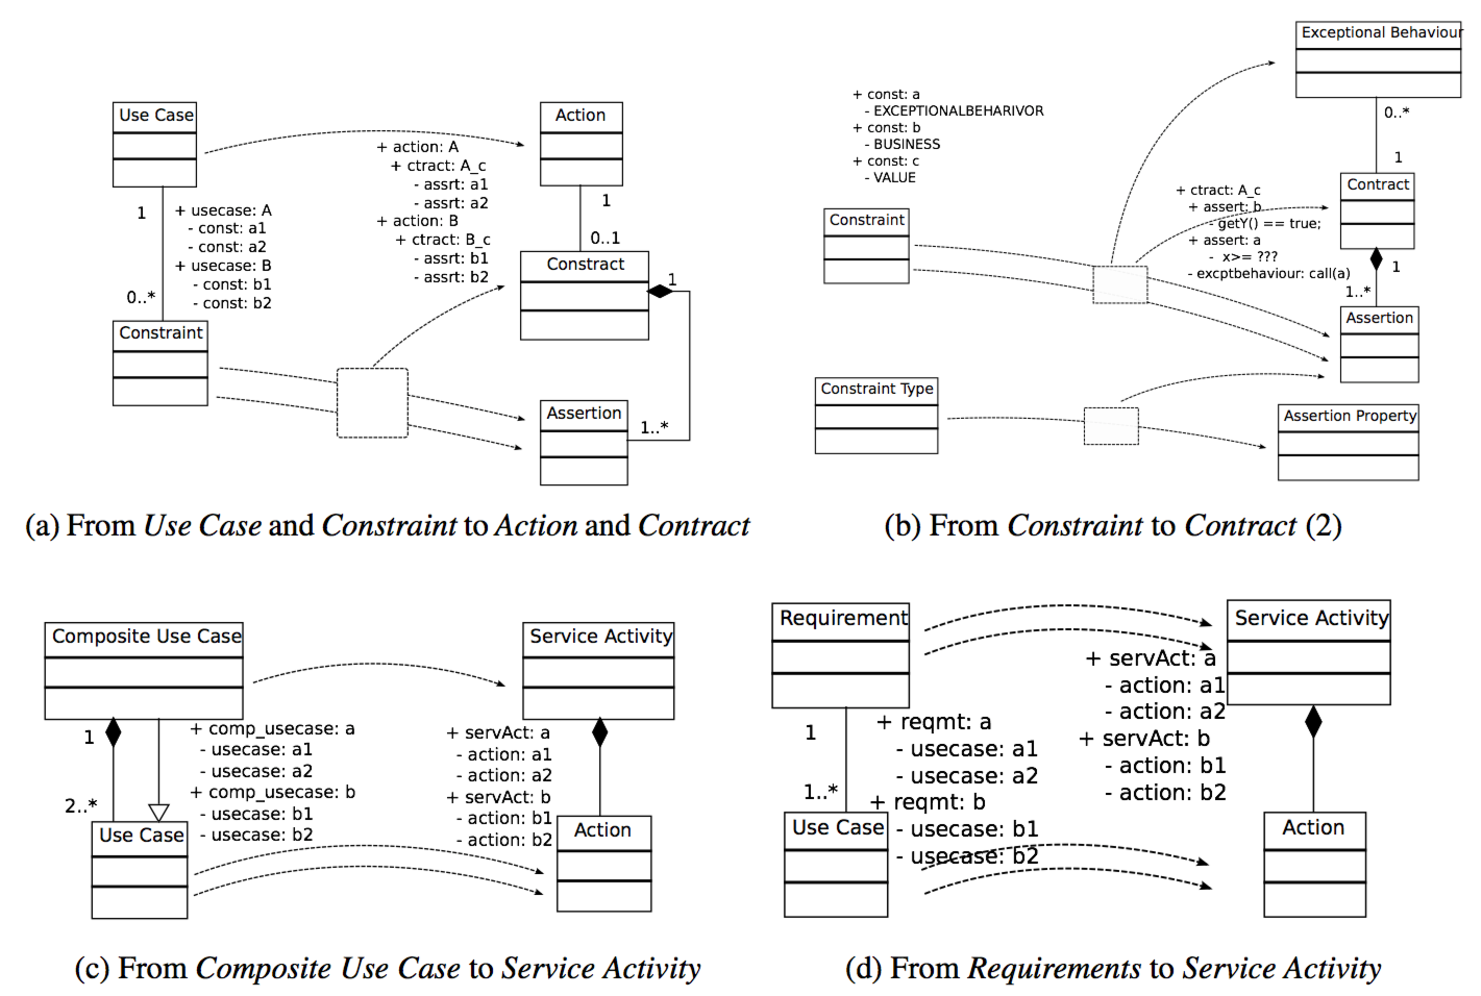
\includegraphics[width=0.96\textwidth]{figs/35}}
%\caption{ $\pi$-UseCase to $\pi$-ServiceProcess transformation rules}
%\label{fig:transformationsUseCase-ServiceProcessRules}
%\end{figure}

A {\sf Constraint} associated to a {\sf Use Case}  is transformed into an  {\sf Assertion}.  
The set of resulting assertions  are grouped into a {\sf Contract}.
Constraints are transformed according to their type:
{\sc Business} constraints and {\sc Value} constraints with the {\sf  isExceptionalBehaviour} attribute set to false are transformed into {\sf Assertion}s;
{\sc Value } constraints with the {\sf  isExceptionalBehaviour} attribute set to true are transformed into {\sf Exceptional behaviour}s.

In order to transform constraints of type {\sf Value Constraint}, the designer must specify thresholds to be associated to the assertions of a contract.
By default, value constraints are transformed into pre-conditions and business constraints are transformed into post-conditions. 
  
%A {\sf Requirement} and a {\sf Composite use case} in a  $\pi$-UseCase model are transformed respectively into a {\sf Service activity} and an {\sf Action} (see figures  \ref{fig:transformationsUseCase-ServiceProcessRules}-c  and d). 
%
%
%\begin{figure}
%\centering{
%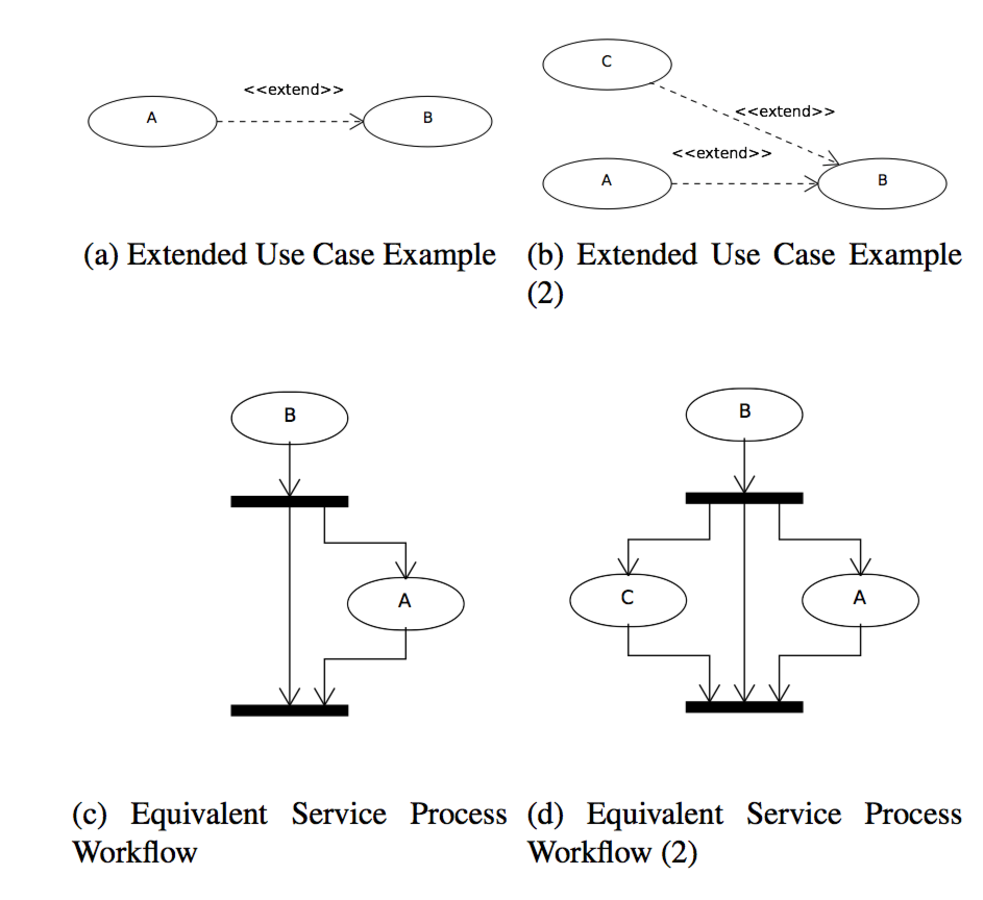
\includegraphics[width=0.80\textwidth]{figs/37}}
%\caption{ Extended Transformation Examples}
%\label{fig:transformaton-examples}
%\end{figure}

%The transformations for {\sc Extend} and {\sc Include} dependencies  are not as simple as the previous transformations (figures \ref{fig:transformaton-examples}-a). 

The relationships of type  {\sc Extend} and {\sc Include}  determine the way the business process is expressed as a workflow.  
The generated workflow is composed by {\sf Fork} and {\sf Join} nodes,  {\sc Control flow} constructors, as well as entities of type {\sc Action}.

%\begin{figure}
%\centering{
%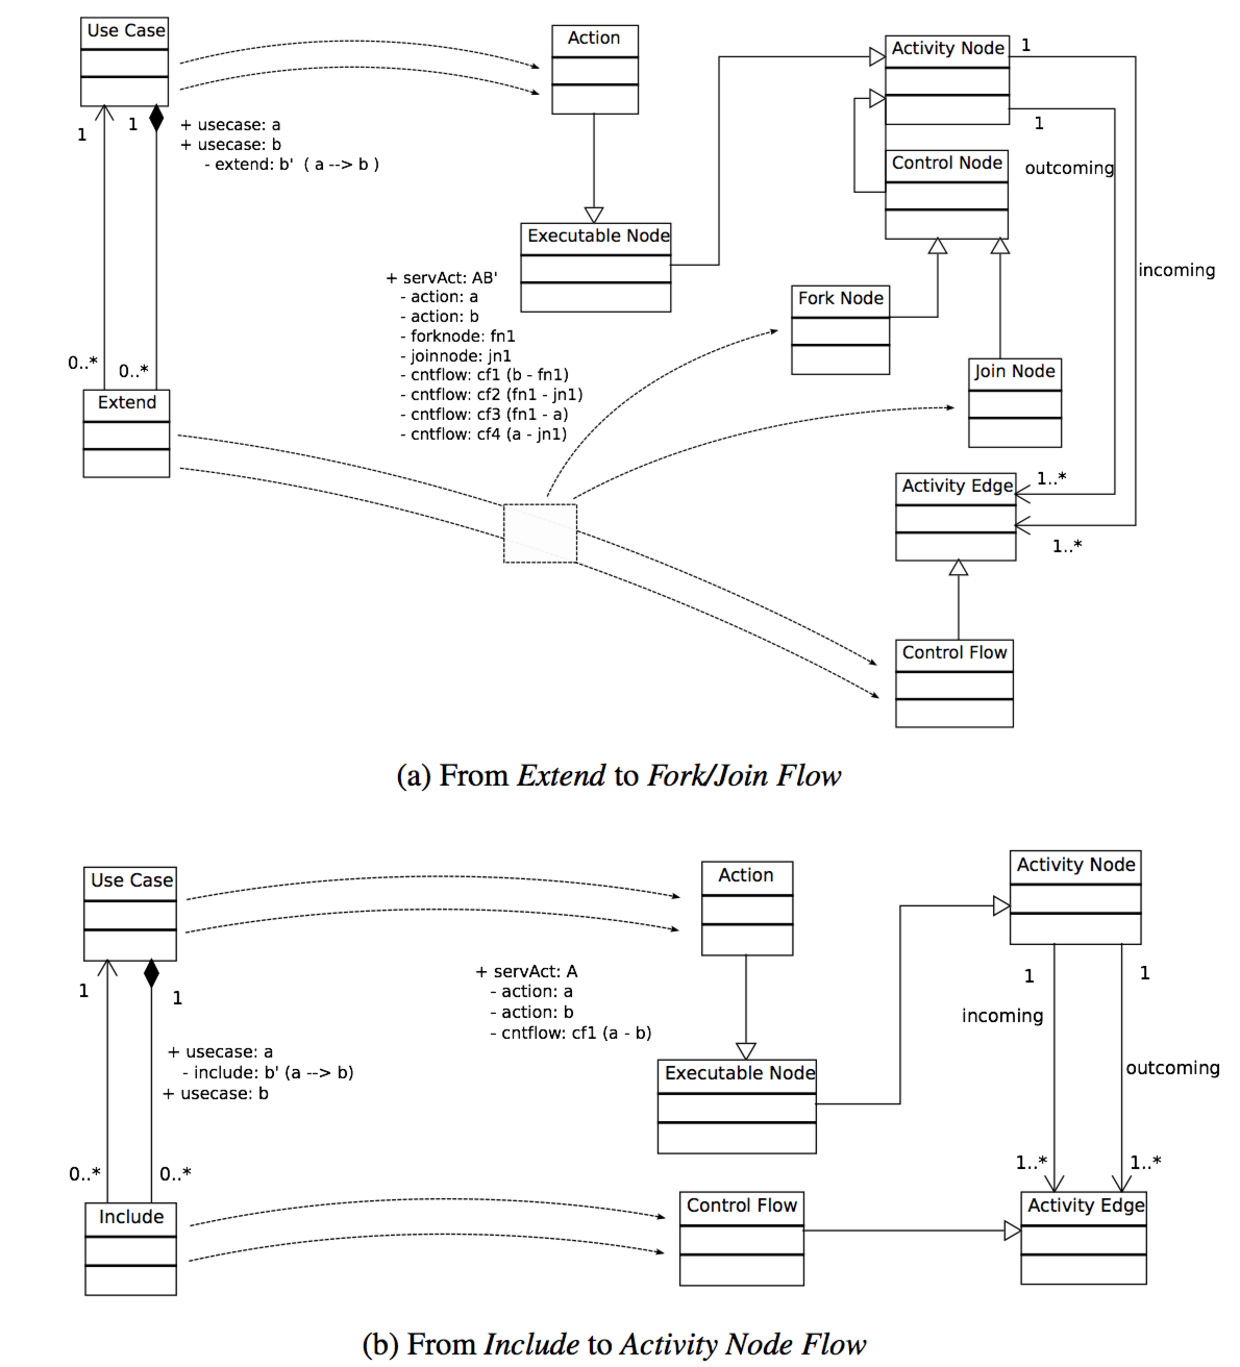
\includegraphics[width=0.96\textwidth]{figs/36}}
%\caption{ $\pi$-UseCase to $\pi$-ServiceProcess Model Transformation Rules (2)}
%\label{fig:transformationsUseCase-ServiceProcessRules}
%\end{figure}

{\sf Include} use case entities are transformed into an {\sf Action} sequence.
A {\sc Use case} element is transformed into an {\sf Action}. 
A set of $n$ {\sc Use cases} is transformed into an  $n-1$ {\sf Object flow} elements. 

The details of these transformations are not included here (due to space restrictions).
They can be found in~\cite{SouzaNeto:2012}.

\begin{example}[To Publish Music \textit{(cont)}]\label{ex:toPublicMusicT1}
The rules presented above have been applied to the model in Figure~\ref{fig:piUseCaseModel}, in order to obtain the $\pi$-Service Process model for our running example (Figure~\ref{fig:CIM:serviceprocess}).

The ``listen music'' use case is transformed into a Service Action. 
This Action  represents a Spotify service function that can be invoked to play the music. 
For the ``publish music'' use case,  constraints are transformed into a set of assertions that are grouped into a Contract ({\sf ``publishMusicContract''}) associated to the Action {\sf ``publishMusic''}. 
The ``download music'' use case  includes the payment process to buy the music. 
Thus, these use cases  are transformed into {\sf Actions}, and a {\sf Service Activity} that aggregates these {\sf Actions}.   
This \textsf{Service Activity} is transformed into a sequence flow on the $\pi$-service process model.
%(as shown in figure \ref{fig:transformation-example-include}). 
The same rule is applied for the ``publish music'' use case, which has two extended use cases, to publish on Twitter and Facebook.
 \end{example}

%\begin{figure}
%\centering{
%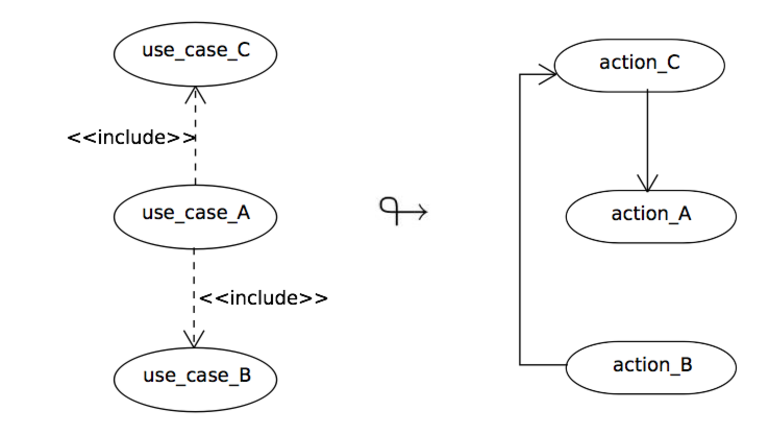
\includegraphics[width=0.76\textwidth]{figs/38}}
%\caption{ Include Transformation Example}
%\label{fig:transformation-example-include}
%\end{figure}

% _ . _ . _ . _ . _ . _ . _ . _ . _ . _ . _ . _ . _ . _ . _ . _ . _ . _ .
\subsection{From $\pi$-ServiceProcess to $\pi$-ServiceComposition}
% _ . _ . _ . _ . _ . _ . _ . _ . _ . _ . _ . _ . _ . _ . _ . _ . _ . _ .

The  principle of the transformation  of a  $\pi$-Service Process model into a $\pi$-Service Composition model is to group {\sf Contracts} into {\sf A-Policies} and {\sf Actions} into {\sf Service Activities}.   

Each {\sf Assertion} of a {\sf Contract} is transformed into a {\sf Rule}. 
{\sf Rules}  concerning the same NFP  are grouped into {\sf A-Policies}. 
Each {\sf Assertion} of a {\sf Contract} is transformed into a {\sf Rule:Condition} attribute. 
If the {\sf Assertion} has a value type, the name and the attributes are transformed into {\sf Variables} in the target model.  
The {\sf Assertion: aProperty} attribute can have different transformations, according to: 
\textit{(i)} a {\sf Precondition} is transformed into {\sf Pre};
\textit{(ii)} a {\sf Post-Condition} is transformed into a {\sf  Post};
\textit{(iii)} a {\sf TimeRestriction} is transformed into {\sf Time}.

%
%\begin{figure}
%\centering{
%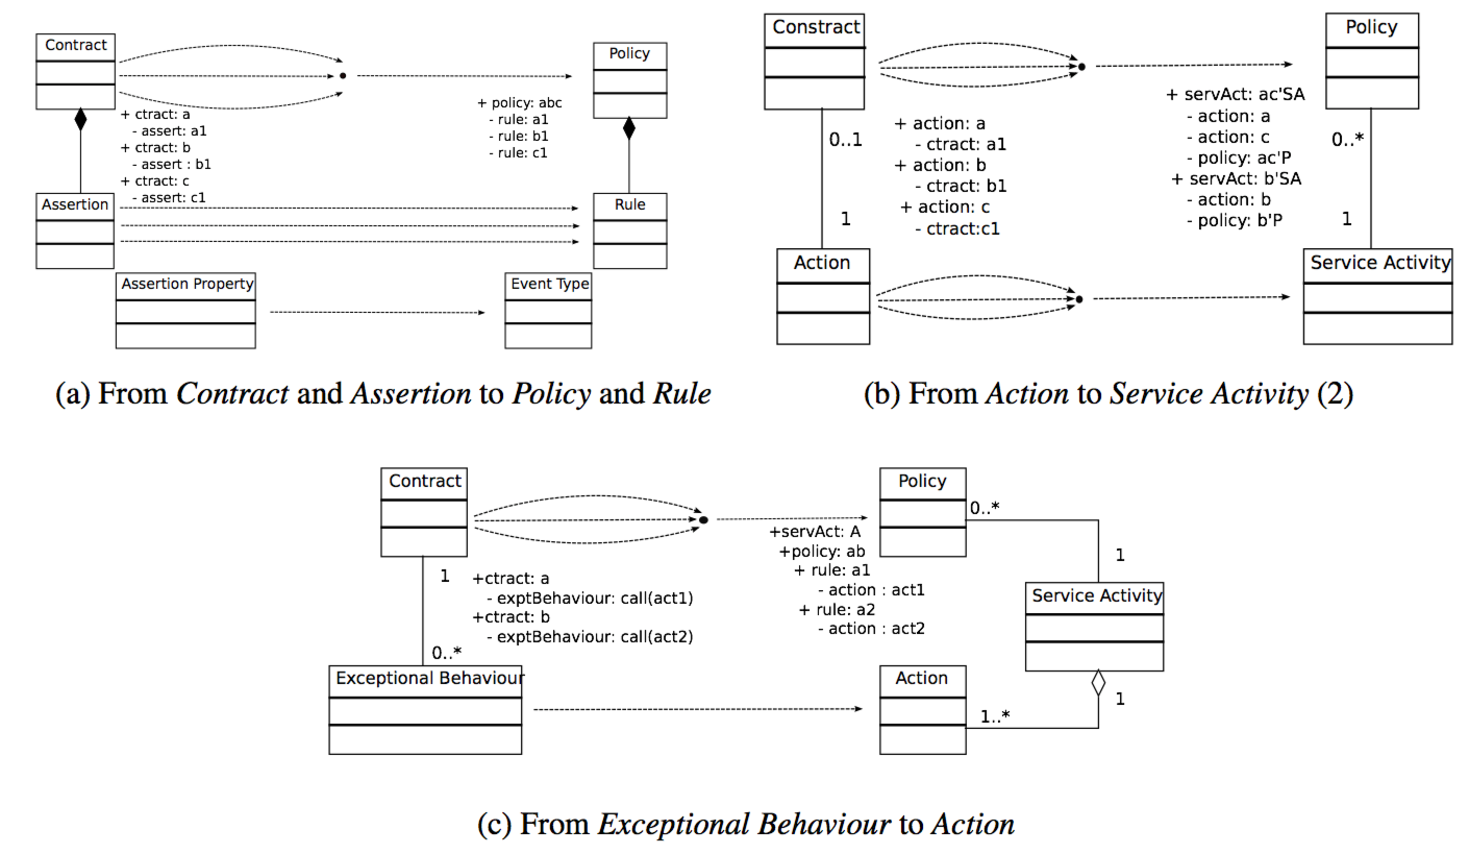
\includegraphics[width=0.96\textwidth]{figs/ExceptionalRules}}
%\caption{$\pi$-ServiceProcess to $\pi$-ServiceComposition Model Transformation Rules}
%\label{fig:ServiceProcess-ServiceComposition-Rules}
%\end{figure}
{\color{red}
A {\sf Package} in the $\pi$-use case model is transformed   into a {\sf Business Collaborator}. 

Placido: Is this correct? Why it is here? We consider the $\pi$-use case in the previous section!
}

{\sf Actions} and {\sf Service activity} of a $\pi$-Service Process model are transformed into their homonym concepts of the $\pi$-Service Composition model. 

An {\sf Exceptional behaviour} entity is transformed into an {\sf Action} in a $\pi$-Service Composition model and every {\sf Non-functional attribute} associated to an element ({\sf Contract} or {\sf Non-functional requirement}) in a $\pi$-service process model becomes a {\sf Non-functional attribute} associated to the corresponding element {\sf A-Policy} in a $\pi$-service composition model.\footnote{\color{red} Not found in the metamodel! --Martin and Umberto}
Finally, {\sf Actions} are grouped by  a {\sf Business collaborator}.\footnote{\color{red} How? Where in the metamodel? --Martin and Umberto} 

%\begin{figure}
%\centering{
%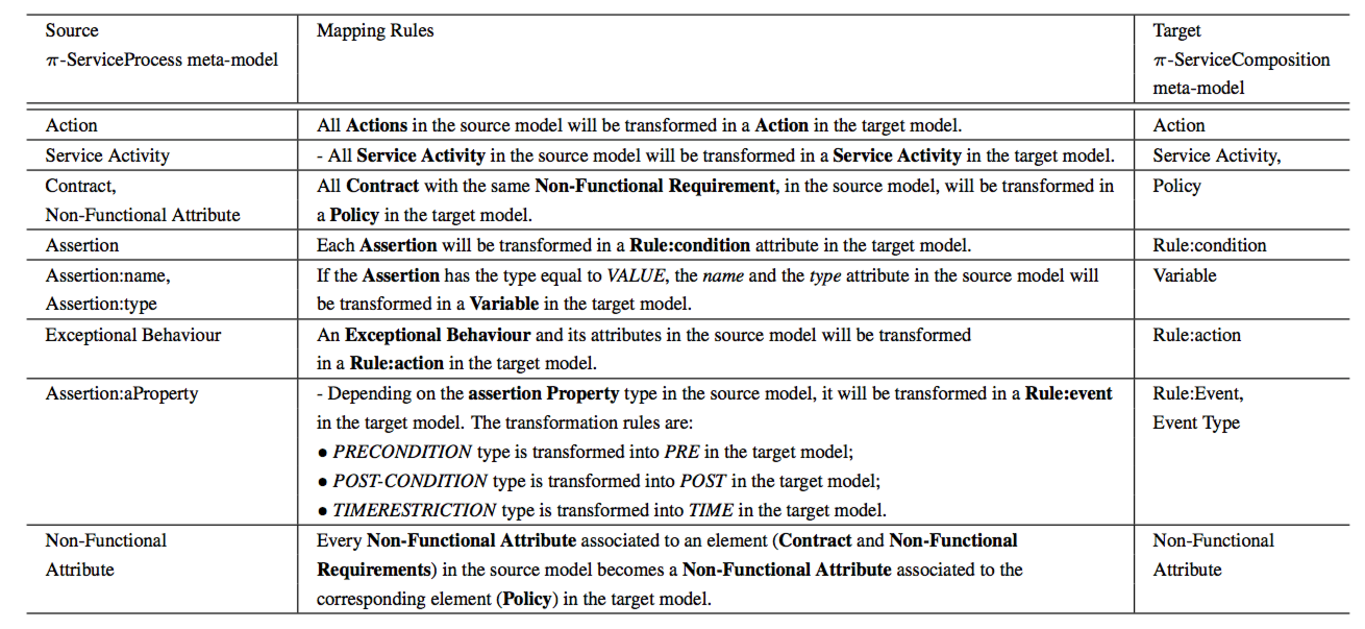
\includegraphics[width=1\textwidth]{figs/ServiceProcess-ServiceComposition}}
%\caption{ Transformation Rules: From $\pi$-ServiceProcess to $\pi$-ServiceComposition}
%\label{fig:ServiceProcess-ServiceComposition}
%\end{figure}






%As the $\pi$-ServiceComposition model refines the $\pi$-ServiceProcess concepts at PIM level, a service previously defined as actions (source model) is refined as composition of those actions (target model) that are necessary to represent a business service, identifying who are the partners involved in the realization ({\sc Business collaborators}). 
%In addition, $\pi$-SOD-M defines a platform specific model based on web services composition. This model is explicitly indicates those actions which are (or will be, if not yet implemented) supported by web services.

\begin{example}[To Publish Music \textit{(cont)}]\label{ex:toPublicMusicT5}
Considering the example scenario, the model in Figure~\ref{fig:PiServiceCompositionModel} was obtained by applying the rules above to the model depicted by Figure~\ref{fig:CIM:serviceprocess}.  

The "securityLoginPolicy" consists of a set of {\sf Rules} that were transformed from the {\sf Assertions} in $\pi$-service process model. 
The information about Facebook and Spotify (both of them {\sf Business Collaborators}) come from entity of type {\sc Package} in the $\pi$-use case model.\footnote{\color{red} Como assim? - Placido, explain this, please! Why have we bypassed one level here?}
\end{example}

% _ . _ . _ . _ . _ . _ . _ . _ . _ . _ . _ . _ . _ . _ . _ . _ . _ . _ .
\subsection{From $\pi$-ServiceComposition to $\pi$-PEWS}
% _ . _ . _ . _ . _ . _ . _ . _ . _ . _ . _ . _ . _ . _ . _ . _ . _ . _ .

This section describes the PIM to PSM transformations from a $\pi$-Service composition model to a $\pi$-PEWS model. 
We distinguish two groups of rules: \textit{(i)} those transforming service composition entities into workflows; and \textit{(ii)} those that transform  A-Policies into Contracts.

Single actions (represented by {\sf Action} and {\sf Action:name}\footnote{\color{red} Where is the name defined?}) are transformed into individual service {\sf Operations}. 
Complex actions (represented by {\sf ServiceActivity}  and  {\sf ServiceActivity:name}\footnote{\color{red} Where is the name defined?}) are transformed into (named) composite operations that defines a (named) workflow of the application. 
Composition patterns expressed using the operators {\sc\em merge, decision, fork and join} are transformed into their corresponding workflows of the $\pi$-PEWS model.

%\begin{figure}
%\centering{
%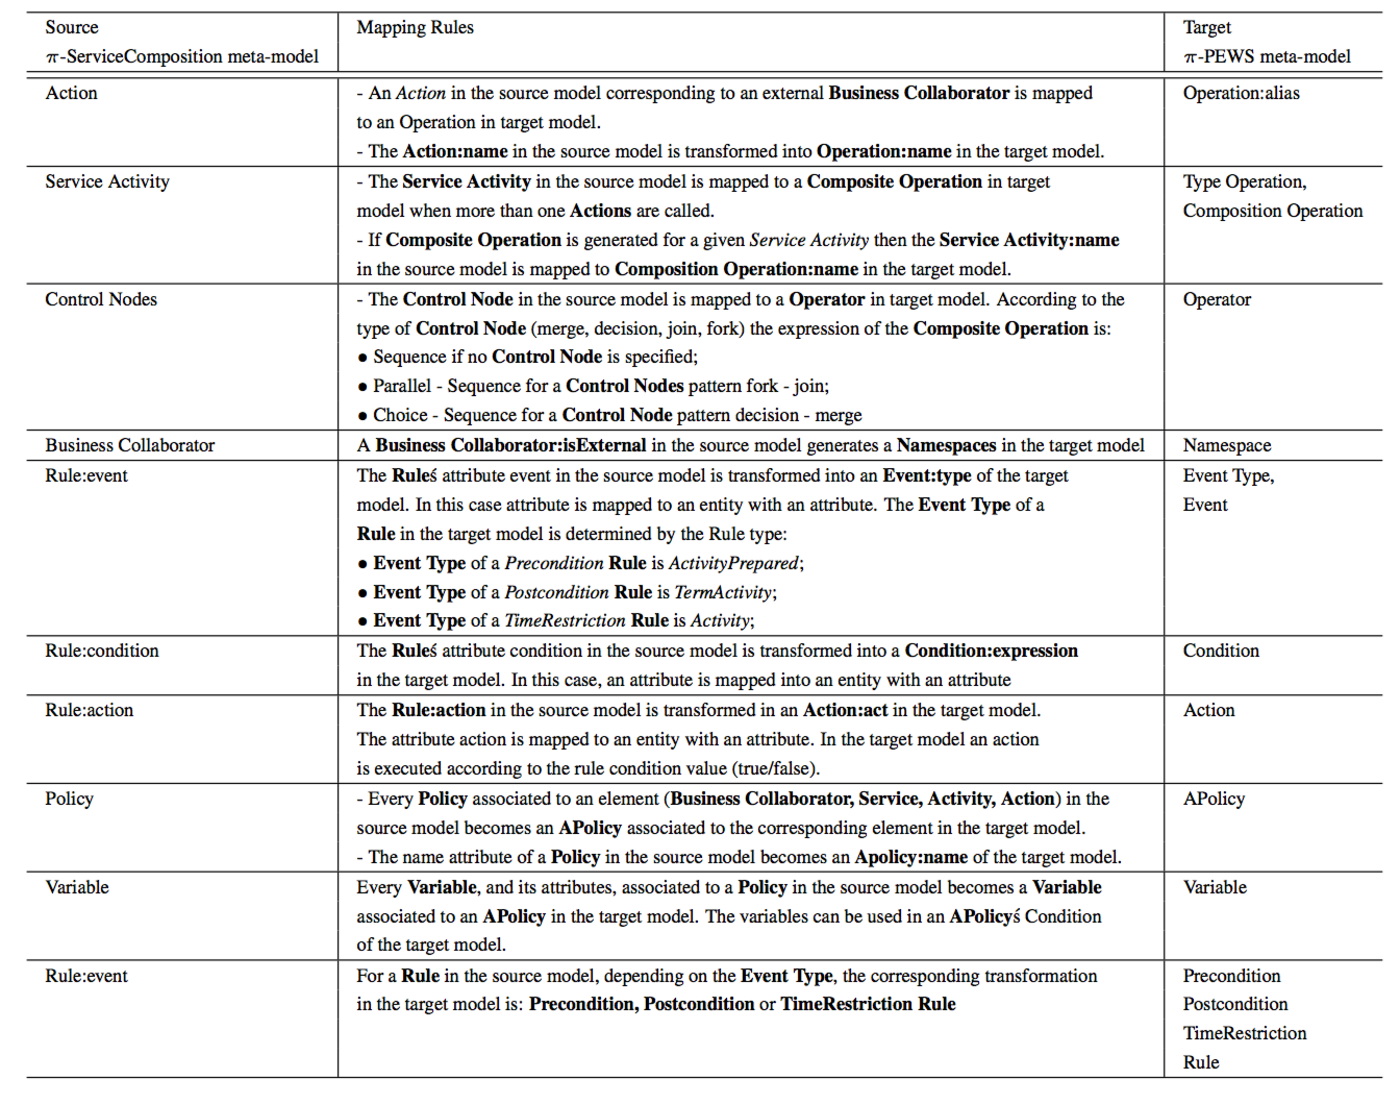
\includegraphics[width=0.96\textwidth]{figs/Table7}}
%\caption{Transformation Rules: From $\pi$-ServiceComposition to $\pi$-PEWS}
%\label{fig:ServiceComposition-Pews-Rules}
%\end{figure}

The A-Policies defined for the entities of a $\pi$-service composition model are transformed into {\sf A-policy}
\footnote{\color{red} Please rename this for CONTRACT on the pi-pews metamodel!} 
entities, named according to the names expressed in the source model. 
The transformation of the rules expressed in a $\pi$-service composition is guided by the event types associated to these rules. 
The variables associated to an A-Policy expressed in a $\pi$-service composition model as {\sf $<$Variable:name, Variable:type$>$} are transformed into entities  {\sf Variable} with attributes {\sf Name} and {\sf Type} directly specified from the elements {\sf Variable:name} and {\sf Variable:type} of a $\pi$-service composition model.

Events of type {\sf Pre}, {\sf Post} and {\sf Time} generate, respectively, {\sf Preconditions}, {\sf Postcondition} and {\sf TimeRestrictions}.

\begin{example}[To Publish Music \textit{(cont)}]\label{ex:toPublicMusicT6}
Figure \ref{fig:piSOD-M} shows the $\pi$-PEWS code resulting from the $\pi$- service composition model  of our scenario example.
\end{example}


\subsection{Implementation}
We have provided tools for aiding the user to define and transform the models for all the levels, except for the CIM into PIM level, which should be manually performed.

Our tool is implemented as a series of Eclipse plug-ins: 
\begin{itemize}
\item 	We  used the Eclipse Modeling Framework (EMF)\footnote {The EMF project is a modeling framework and code generation facility for building tools and other applications based on a structured data model.}   for implementing the  $\pi$-Service Composition and $\pi$-{\sc Pews}  meta-models. 
Then, from these meta-models, we  developed plug-ins to support their graphical representation.

\item	 We used  ATL\footnote{http://eclipse.org/atl/. An ATL program is basically a set of rules that define how source model elements are matched and navigated to create and initialize the elements of the target models.}
for implementing the  mappings between models.

\item 	We  used Acceleo\footnote{http://www.acceleo.org/pages/home/en} for implementing  the code generation plug-in for generating executable code. 
It takes a $\pi$-PEWS model and generates the code to be executed by the {\em A-Policy} based service composition execution environment\footnote{\color{red} Placido: Policy or contract??.}. 
\end{itemize}

